%======================================================================
\chapter{Applications}
%======================================================================
\section{Visualization}
\begin{figure}[h]
\begin{center}
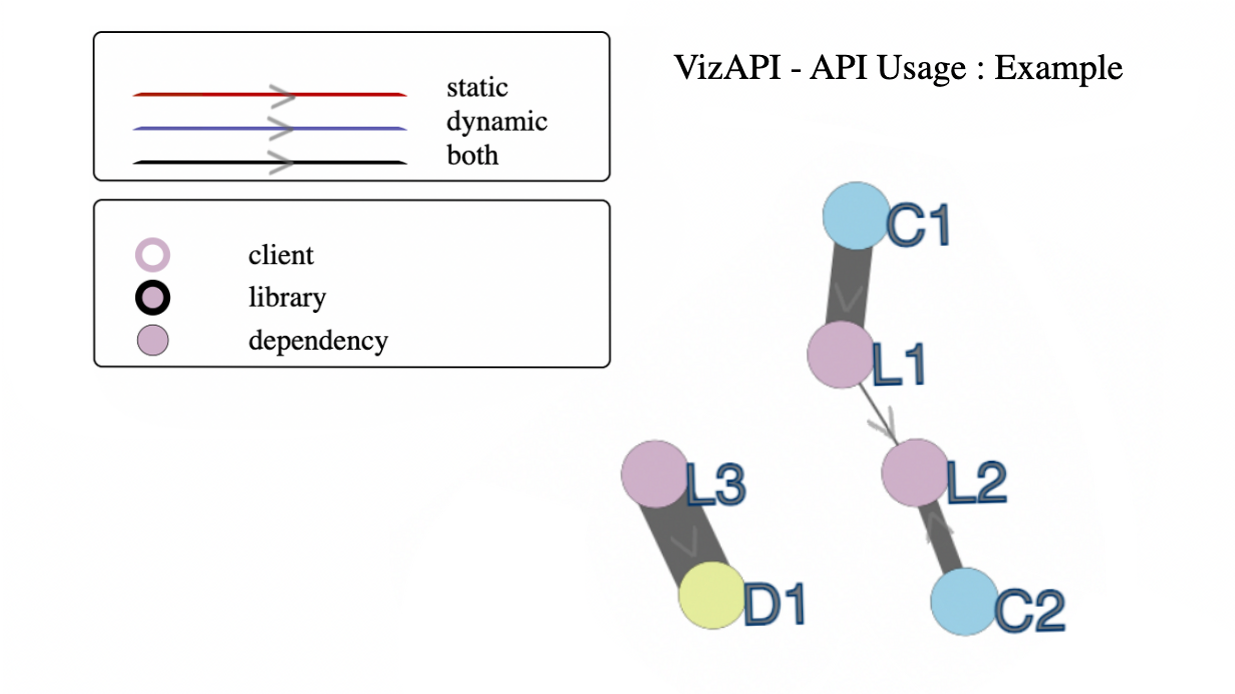
\includegraphics[height=6cm]{images/intro-example.png}
\caption{An Example VizAPI Application}
\label{fig:example}
\end{center}
\end{figure}


Figure~\ref{fig:example} illustrates a possible VizAPI usage scenario, from the perspective of a client developer. Consider a client $C$ (blue nodes) and a library $L$ (purple nodes), in the context of plain Java. Library $L$ has packages $L_1$, $L_2$, and $L_3$. $C$ calls into $L_1$ and $L_2$. Internally, within $L$, $L_1$ and $L_2$ call into each other, but not into $L_3$. The VizAPI result, with no edges from $C$ directly to $L_3$, allows a developer to conclude that breaking changes in $L_3$ will not affect $C$. Also, if only $L_3$ uses an external dependency $D$ (yellow node), then we know that $C$ will not need $D$ to be on its classpath.

From the library developer side, under plain Java (i.e. no runtime containers) and considering reflection, the potential API surface of any component is huge. Essentially: every method can be called, and every field can be read and written. Even considering only the published API surface (methods, fields, classes, and annotations with the correct visibility modifiers), libraries' API surfaces still often have hundreds to thousands of members. The breadth of the API surface is a liability with respect to continued maintenance of the library; many developers aspire to avoid breaking changes by preserving, whenever possible, library behaviour that is depended on by clients. Knowing that few clients use a particular API would be valuable.

On the other hand, we would expect (and have verified in other work) that each client uses only a small portion of each of its dependencies' API surfaces. Consider breaking changes again. GitHub provides the Dependabot tool~\cite{mullans20:_keep_depen}, which monitors for upstream changes and automatically proposes pull requests to update dependency versions. That tool may well pull in breaking changes. However, we hypothesize that, most of the time, most breaking changes will not affect most clients; it is useful for clients to know whether they are using the parts of the API surface that are subject to a particular breaking change. A client with broad dependencies on a library (uses a larger fraction of its API surface) is more likely to be affected by its changes than a client with narrow dependencies (smaller fraction). A narrow library dependency would also suggest that it would be easier to swap the library for a functionally similar replacement.

Additionally, as researchers, we would like to understand how library
APIs are used by clients more generally. Zhong and
Mei~\cite{zhong19:_empir_study_api_usages} investigated API usages in
a dataset of 7 experimental subjects (clients) and the libraries that
they depend on.  They found that clients use less than 10\% of the
declared APIs in libraries. Our visualization allows developers and
researchers to visualize distribution information about how different
parts of clients use different parts of libraries.

This paper presents the VizAPI tool, which shows visualization overviews showing API usages---from clients to libraries, but also between libraries (including transitive dependencies). VizAPI incorporates information from static and dynamic analyses. 
We have made VizAPI publicly available, although it is still in development:
\begin{center}
\url{https://github.com/SruthiVenkat/api-visualization-tool}
\end{center}

Our contributions include:
\begin{itemize}
\item an implementation of the VizAPI tool, which presents a visualization of API usage information; VizAPI collects static information and instruments Java code and collect dynamic instrumentation information about API uses in practice and presents it as a d3 visualization (Section~\ref{subsec:collecting-data}--\ref{subsec:vis-system});
\item a discussion of VizAPI usage scenarios (Section~\ref{subsec:evaluation}) based on a collection of 11 libraries and 38 clients.
\end{itemize}


\section{Library Fission}
Modern software uses libraries extensively, to reuse functionality. Over time, libraries tend to extend their functionality, introduce more features and modify existing ones. This could lead to huge library sizes, a lot of which goes unused by a client that imports it. This is called software bloating and there has been work around debloating. Debloating focuses on the client’s execution and analyzing the client. We propose library fission, which focuses on splitting libraries based on client usage. This is a more permanent solution to bloating and does not require running analyses on clients for every execution. (We aim to split libraries based on client behaviour in a way that sub-modules of the fissioned library have common functionality.)

\section{Upgrades, Breaking Changes and Backward Compatibility}
Library developers can observe different usage patterns of their APIs. The clusters observed in library packages can help with new version releases. Breaking changes might be restricted to clusters and library developers can choose whether to make clusters from new versions backward compatible with other clusters from older versions or not. Clients can also check if breaking changes in new library versions will affect their code during upgrades. 